\section{Introduction}

In this project, we will look at a classic of scientific computing, namely ballistics calculations. Our setup is as follows. A cannonball of weight 6kg is fired from the origin with an initial speed of 450m$\text{s}^{-1}$ and at an angle $\theta$, as shown in the figure below. For simplicity, we will ignore the size of the cannonball.

\begin{center}
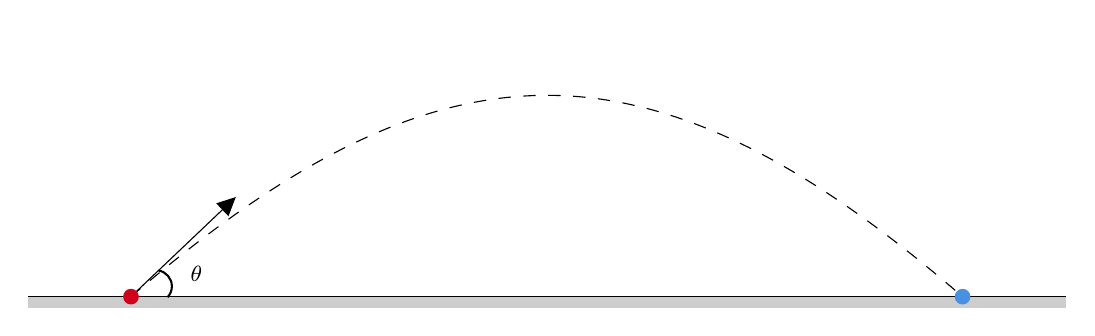
\begin{tikzpicture}[x=0.75pt,y=0.75pt,yscale=-1,xscale=1]
% Straight Lines [id:da6525233007371856] 
\draw    (80.33,110) -- (580.33,110) ;
% Shape: Rectangle [id:dp5452175321360211] 
\draw  [draw opacity=0][fill={rgb, 255:red, 155; green, 155; blue, 155 }  ,fill opacity=0.5 ] (80.33,110) -- (580.33,110) -- (580.33,115.33) -- (80.33,115.33) -- cycle ;
% Shape: Circle [id:dp4676081231695395] 
\draw  [color={rgb, 255:red, 74; green, 144; blue, 226 }  ,draw opacity=1 ][fill={rgb, 255:red, 74; green, 144; blue, 226 }  ,fill opacity=1 ] (527,110) .. controls (527,108.07) and (528.57,106.5) .. (530.5,106.5) .. controls (532.43,106.5) and (534,108.07) .. (534,110) .. controls (534,111.93) and (532.43,113.5) .. (530.5,113.5) .. controls (528.57,113.5) and (527,111.93) .. (527,110) -- cycle ;
% Curve Lines [id:da8791670265718843] 
\draw  [dash pattern={on 4.5pt off 4.5pt}]  (129.83,110) .. controls (280.33,-19.33) and (380.33,-19.33) .. (530.5,110) ;
% Straight Lines [id:da4007655115472968] 
\draw    (129.83,110) -- (178.16,64.07) ;
\draw [shift={(180.33,62)}, rotate = 496.45] [fill={rgb, 255:red, 0; green, 0; blue, 0 }  ][line width=0.08]  [draw opacity=0] (8.93,-4.29) -- (0,0) -- (8.93,4.29) -- cycle    ;
% Shape: Arc [id:dp7717720335135645] 
\draw  [draw opacity=0][line width=0.75]  (143.2,97.42) .. controls (146.79,98.06) and (149.52,101.19) .. (149.54,104.96) .. controls (149.55,107.02) and (148.76,108.88) .. (147.45,110.27) -- (141.84,105) -- cycle ; \draw  [line width=0.75]  (143.2,97.42) .. controls (146.79,98.06) and (149.52,101.19) .. (149.54,104.96) .. controls (149.55,107.02) and (148.76,108.88) .. (147.45,110.27) ;
% Shape: Circle [id:dp9649843290823428] 
\draw  [color={rgb, 255:red, 208; green, 2; blue, 27 }  ,draw opacity=1 ][fill={rgb, 255:red, 208; green, 2; blue, 27 }  ,fill opacity=1 ] (126.33,110) .. controls (126.33,108.07) and (127.9,106.5) .. (129.83,106.5) .. controls (131.77,106.5) and (133.33,108.07) .. (133.33,110) .. controls (133.33,111.93) and (131.77,113.5) .. (129.83,113.5) .. controls (127.9,113.5) and (126.33,111.93) .. (126.33,110) -- cycle ;

\draw (161.33,99) node [font=\footnotesize] {$\theta$};

\end{tikzpicture}
\end{center}


\noindent
Although we have chosen particular parameters for our model, we will generalise our code so that it works for any other reasonable parameters. That is, we will decouple our chosen model parameters from the implementation itself, so that we can easily adapt our model when the requirements change. The complete source code is listed in the appendix.